\section{Today’s assignment}
Today's class will be divided in three main parts. First we will learn the main algorithmic principle behind deep learning and code the Backpropagation algorithm in numpy.  Secondly, we will learn the basics of the Theano module for Python, which allows to easily implement deep learning techniques that run on a Graphical Processing Unit (GPU) for optimal speed. Thirdly we will see some more complex deep learning concepts and NLP specific issues.

If you are new to the topic you should aim to finish the deep learning principles part (Ex. 7.1 and 7.2) and at least Ex 7.3 and 7.4 of the Theano part. If you have some spare time have a look at the more complex deep learning issues. If you already know Backpropagation well and have experience with normal Python, you should aim to complete Theano and some or all the exercises of the third part. 

\section{Introduction To Deep Learning and Theano}

Deep learning is the name behind the latest wave of successful neural network research, a very old topic dating from the first half of the XX century. Deep learning techniques have attained formidable impact in the machine learning community, in particular in the fields of image, speech processing and NLP. Some of the changes that led to this renewed success reside not only in the improvements on the existing neural network algorithms but also in the amount of data available and the increase in computer power. In particular, the use of Graphical Processing Units (GPUs) has allowed the application of neural networks to very large datasets. Working with GPUs is not trivial as it requires dealing with specialized hardware. Luckily, as it is often the case, we are one Python import away from solving this problem. For the particular case of deep learning, the Theano\footnotemark\footnotetext{http://deeplearning.net/software/theano/} module allows us to express models symbolically, automatically computing gradients and solve overflow problems. Furthermore, the code is also ready to use with CUDA-compatible GPUs.

\section{A Look Back at Log-linear Models from Day One} 

\subsection{Log-linear models as composition of linear and non-linear functions}

There is nothing particularly difficult in the deep learning concept. You have already visited all the mathematic principles you need in the first days of the labs of this school. The core element in deep learning is the multi-layer perceptron (MLP) architecture. This is basically a non-linear model built by composing linear and non-linear transformations. This can be seen as a composition of two or more log-linear models, like the ones we saw on Day 1. For this reason, to introduce the topic we are going to start with one single log-linear model and progress from that point on.

Recall the maximum entropy classifier in Section \ref{s:me}. This method used a simple log-linear model to define the probability that an input vector represented by a vector of features $\boldsymbol{f}(x,y)$, belongs to a each of $K$ possible classes $y_k$. For the purpose of introducing deep learning, a more general form here given by 
%
\begin{equation}
p(y_k|\mathbf{x}) = \frac{\exp(\mathbf{W}_k \cdot \mathbf{x} + w_k)}{Z(\mathbf{W},\mathbf{w},\mathbf{x})} = \frac{\exp(\mathbf{W}_k \cdot \mathbf{x} + w_k)}{\sum_{1=k'}^K \exp(\mathbf{W}_{k'} \cdot \mathbf{x} + w_{k'})}. 
\label{eq:loglineargen}
\end{equation}
%
Keep in mind that this is just a discrete probability distribution over $K$ classes. There are some differences with respect to  Eq:\ref{eq:loglinear}. We have not only weights $\mathbf{W} \in \mathbb{R}^{K \times I}$ but also a bias $\mathbf{w} \in \mathbb{R}^{K \times 1}$. Also $\mathbf{x} \in \mathbb{R}^{I \times 1}$, rather than being restricted to binary features $\boldsymbol{f}(x,y)$. As we will see later, this more general model can still be trained with Stochastic Gradient Descent (SGD), described in Section \ref{s:me}.    

\noindent Now, lets rewrite this log-linear model as a composition of a generic linear transformation 

\begin{equation}
\mathbf{z} = \mathbf{g}(\mathbf{x}) = \mathbf{W} \cdot \mathbf{x} + \mathbf{w}
\label{eq:linear}
\end{equation}

\noindent where $\mathbf{z} \in \mathbb{R}^{K \times 1}$ and the softmax non-linear transformation.

\begin{equation}
\tilde{z}_k = f_k(\mathbf{z}) = \frac{\exp(z_k)}{\sum_{1=k'}^K \exp(z_{k'})}. 
\label{eq:softmax}
\end{equation}

\noindent It it easy to see that this leads to the same model as Eq:\ref{eq:loglineargen}, since

\begin{equation}
p(y_k|\mathbf{x}) = \tilde{z}_k = (f_k \circ \mathbf{g})(\mathbf{x}). 
\end{equation}

\noindent In other words, the probability of class $k$ is given by the $k$-th output of the softmax.

\begin{figure}
\centering
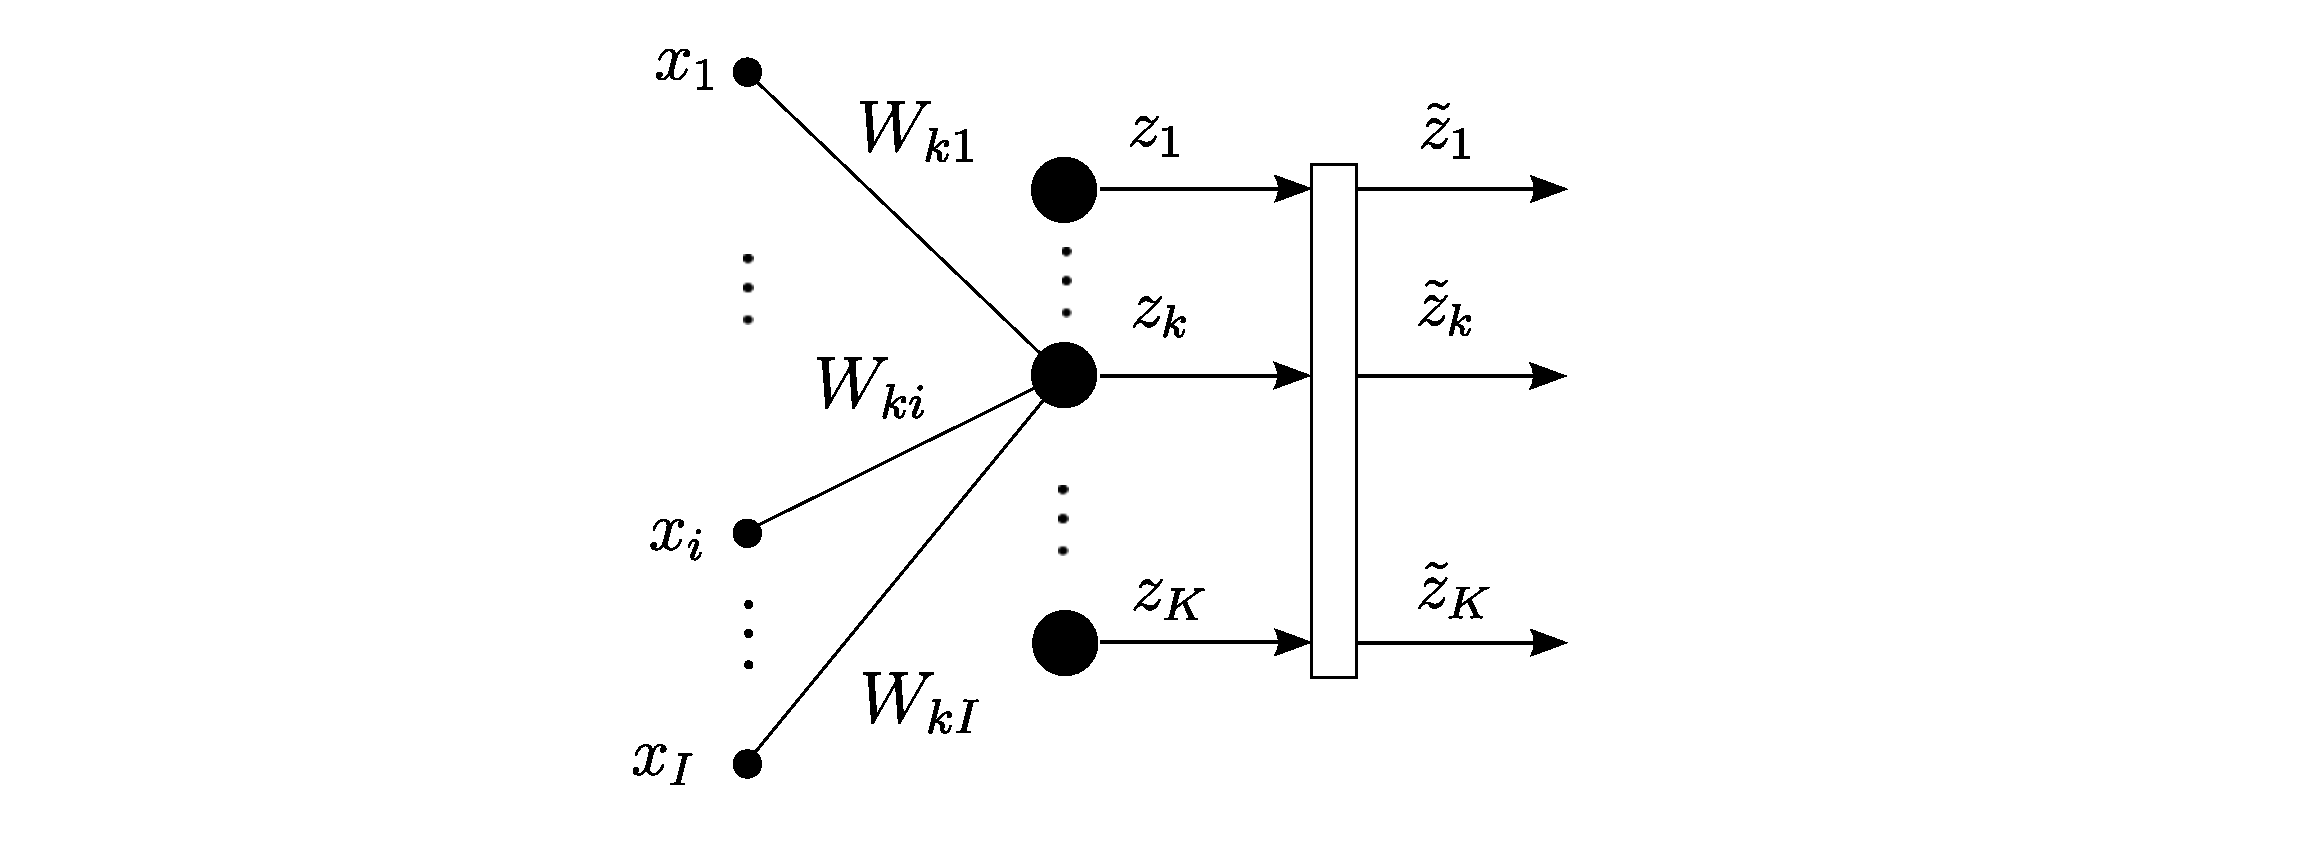
\includegraphics[scale=0.4]{figs/deep_learning/LayerP.pdf}
\caption{Representation of a log-linear model as a composition of a linear and a non-linear transformation. Left: Detail of dependencies of the $k$-th output on the input features $\mathbf{x}$. Right: Simplified representation using vectors.}
\label{fig:LayerP}
\end{figure}

\subsection{Deriving SGD for compositions of functions: The Chain Rule}

As we saw on day one, these models can be trained by  stochastic gradient descent (SGD). All we need is to compute the gradient  of the cost $\nabla\mathcal{F}$ with respect to the parameters we wish to estimate. To remain close to the maximum entropy example, we will use the average minus posterior probability of the correct class given the input as cost

\begin{equation}
\mathcal{F}(\mathcal{D};\Theta) = -\frac{1}{M}\sum_{m=1}^M \log P(y^m | \mathbf{x}^m) = -\frac{1}{M}\sum_{m=1}^M (\log f_{k(m)} \circ \mathbf{g})(\mathbf{x}^m)
\label{eq:CostLogPos}
\end{equation}
	
where here $\Theta=\{\mathbf{W}, \mathbf{w}\}$ and $k(m)$ is the index of the correct class in vector $y^m$. 
Bear in mind however that we could pick other cost functions, we will see this once the topic is fully introduced.

For the sake of the introduction to the topic, the cost function is also now also expressed as a composition of a linear and a non-linear function (see right-most equality of Eq \ref{eq:CostLogPos}). This will help us introduce the fundamental element to MLPs and deep learning. Since the cost function is a composition of two functions  $\mathbf{f}(\mathbf{z})$ and $\mathbf{g}(\mathbf{x})$, in order to compute any derivative we can apply the \textit{chain rule}. For example, if we wanted to compute $\nabla_\mathbf{w}\mathcal{F}(\mathcal{D};\Theta)$ we would need each partial derivative of $\log P(y^m | \mathbf{x}^m)$ with respect to weight $W_{kj}$. Thanks to the chain tule, we can express this as

\begin{equation}
\frac{\partial \log P(y^m | \mathbf{x}^m) }{\partial W_{kj}} = \frac{\partial (\log f_{k(m)} \circ \mathbf{g})(\mathbf{x}^m) }{\partial W_{kj}} = \sum_{k'=1}^K\frac{\partial \log f_{k(m)}(\mathbf{z}^m)}{\partial z_{k'}}\frac{\partial z_{k'}}{\partial W_{ki}}.
\label{eq:gradlogPycx}
\end{equation}

In other words, we have divided the problem of computing the derivative of a composition of functions into computing the individual derivatives and then applying the chain rule. This is a great simplifications, as individual derivatives are immediate and often repeat themselves. To illustrate this, lets see the derivatives involved in this calculation: Deriving the softmax in Eq: \ref{eq:softmax} with respect to its input gives us 

\begin{align}
\frac{\partial \log f_{k(m)}(\mathbf{z}^m)}{\partial z_{k}} = 
  \begin{cases}
      1 - \tilde{z}_k^m  &  \mbox{ if } k = k(m)\\ 
      -\tilde{z}_k^m    &  \mbox{ otherwise } 
  \end{cases}. 
  \label{eq:patialSoftmax}
\end{align}

\noindent Deriving the linear layer in Eq:\ref{eq:linear} gives us

\begin{align}
\frac{\partial z_{k'}}{\partial W_{ki}} = 
  &\begin{cases}
      x_i^m  &  \mbox{ if } k = k'\\ 
      0    &  \mbox{ otherwise } 
  \end{cases}.
  \label{eq:partialLinear}
\end{align}

We can now plug these two equations into Eq: \ref{eq:gradlogPycx} to obtain the derivative for $W_{kj}$. Note that the summation over $k'$ disappears due to Eq:\ref{eq:partialLinear}. We will see this happening further on as each linear output $z_i$ only depends of weights $\mathbf{W}_i$. The derivative of the log-posterior for one weight yields 

\begin{align}
\frac{\partial \log P(y^m | \mathbf{x}^m) }{\partial W_{kj}} = 
  &\begin{cases}
     (1 - \tilde{z}_k^m) x_i^m  &  \mbox{ if } k = k(m)\\ 
       -\tilde{z}_k^m x_i^m             &  \mbox{ otherwise } 
  \end{cases}. 
  \label{eq:partialLogP} 
\end{align}

By solving Eq.~\ref{eq:partialLogP} for all $k$ and $l$ and using Eq.~\ref{eq:CostLogPos} we obtain gradient matrix $\nabla_\mathbf{W}\mathcal{F}(\mathcal{D};\Theta) \in \mathbb{R}^{K \times I}$. That is the matrix of partial derivatives for all weights can be expressed as a sum of outer products over the number of training examples $M$  

\begin{equation}
\nabla_\mathbf{W}\mathcal{F}(\mathcal{D};\Theta) = -\frac{1}{M}\sum_{m=1}^M \Big(\mathbf{y}^m - \hat{\mathbf{y}}^m \Big) \cdot \left(\mathbf{x}^m\right)^T  
\label{gradWeigths}
\end{equation}

\noindent where $\mathbf{y}^m$ is the true one-hot representation of the class corresponding to $\mathbf{x}^m$ and 

\begin{equation}
\hat{\mathbf{y}}^m = \tilde{\mathbf{z}}^m =  (\mathbf{f} \circ \mathbf{g})(\mathbf{x}^m)
\label{eq:forwardPass}
\end{equation}

is our predicted class given our current model parameters and $\mathbf{x}^m$, also known as the \textit{forward pass} when using MLP.

\noindent In order to compute the gradient for the bias $w_{k}$  we only need one additional derivative.

\begin{align}
\frac{\partial z_{k'}}{\partial w_{k}} = 
  &\begin{cases}
      1  &  \mbox{ if } k = k'\\ 
      0  &  \mbox{ otherwise } 
  \end{cases} 
  \label{eqn:eqsilonq}
\end{align}
	
\noindent leading to the gradient

\begin{equation}
\nabla_\mathbf{w}\mathcal{F}(\mathcal{D};\Theta) = -\frac{1}{M}\sum_{m=1}^M \Big(\mathbf{y}^m - \hat{\mathbf{y}}^m \Big)   
\label{eq:gradBias}
\end{equation}

\begin{exercise}
Get in contact with the multi-layer perceptron (MLP) class in Numpy and see that for a single layer this is simply a log-linear model. Revisit the sentiment classification exercise of day one. Reformulate train and test data in a way suitable for the exercises of today.  
\begin{python}
# TODO: Better presetation, other corpus?
import numpy as np
import lxmls.readers.sentiment_reader as srs  
scr     = srs.SentimentCorpus("books")
train_x = scr.train_X.T
train_y = scr.train_y[:, 0]
test_x  = scr.test_X.T
test_y  = scr.test_y[:, 0]
\end{python}
%
Load the MLP and SGD code and create a single layer model by specifying the number of inputs, outputs and the type of layer. Note that the number of inputs equals the number of features and the number of outputs the number of classes (2).
%
\begin{python}
# Define MLP (log linear)
import lxmls.deep_learning.mlp as dl
# Model parameters
geometry = [train_x.shape[0], 2]
actvfunc = ['softmax']
# Instantiate model
mlp      = dl.NumpyMLP(geometry, actvfunc)
\end{python}
Put a breakpoint inside of the lxmls/deep\_learning/mlp.py function and debug step by step. Identify the \textit{forward pass} in Eq: \ref{eq:forwardPass} and the computation of the gradients (to be completed in the next execise). 
\begin{python}
# Play with the untrained MLP forward
hat_train_y = mlp.forward(train_x) 
hat_test_y  = mlp.forward(test_x) 
# Compute accuracy
acc_train = sgd.class_acc(hat_train_y, train_y)[0]
acc_test  = sgd.class_acc(hat_test_y, test_y)[0]
print "Untrained Log-linear Accuracy train: %f test: %f"%(acc_train,acc_test)
\end{python}
\end{exercise}

\subsection{Changing the non-linearity}

Before we get into deeper models it also useful to revise the case in which our non-linear function $\mathbf{f}$ is one or more logistic functions

\begin{equation}
\tilde{z}_k = f(z_k)_k = \frac{1}{1+\exp(-z_k)} 
\label{eq:sigmoid}
\end{equation}

One single logistic function corresponds to a particular case of the softmax case we saw previously. That is, the softmax models a categorical distribution over $K$ possible classes, whereas the logistic models a Bernoulli distribution over two classes. We can however use $K$ logistic function outputs providing us a distribution of $K$ Bernoulli variables, that is, a distributions over strings of bits. We can easily derive the gradients using a similar cost function as the last time, but for now we will limit ourselves to keeping in mind the partial derivative of the sigmoid 

\begin{equation}
\frac{\partial \log f_{k}}{\partial z_{k}} = \tilde{z}_{k} (1-\tilde{z}_{k}).
\label{eq:partsigmoid}
\end{equation}

\noindent This will be helpful in the future.

\section{Going Deeper than Log-linear by using Composition}

\subsection{The Backpropagation Recursion}

We have seen that just using the chain rule we can easily compute gradients for compositions of two functions (one non linear and one linear). However, there was nothing in the derivation that would stop us from composing more than two functions. Lets imagine a general case in which we compose $N$ pairs of non-linear and linear functions.

\begin{equation}
p(y_k|\mathbf{x}) = (f_k^N \circ \mathbf{g}^N \circ \mathbf{f}^{N-1} \circ \mathbf{g}^{N-1} \circ \cdots \mathbf{f}^1 \circ \mathbf{g}^1)(\mathbf{x}),
\end{equation}

\noindent we will call each composition of a linear function

\begin{equation}
\mathbf{z}^n = \mathbf{g}^n(\tilde{\mathbf{z}}^{n-1}) = \mathbf{W}^n \cdot \tilde{\mathbf{z}}^{n-1} + \mathbf{w}^n 
\end{equation}

\noindent and a non-linear function 

\begin{equation}
\tilde{\mathbf{z}}^n = \mathbf{f}^n(\mathbf{z}^n),
\end{equation}

expressed as $(\mathbf{f}^n \circ \mathbf{g}^n)$, a \textit{layer}. All the internal (hidden) layers are going to be sigmoid functions as in Eq: \ref{eq:sigmoid} and $\mathbf{f}^N$ will be a softmax, so that the final output can be interpreted as a distribution over $K$ classes. The parameters of our model are going to be the weights and bias of each layer $\Theta=\{\mathbf{W}^1, \mathbf{w}^1, \cdots \mathbf{W}^N, \mathbf{w}^N\}$.  

If we follow the same steps as in the previous section. Our cost function for SGD will look like this

\begin{equation}
\mathcal{F}(\mathcal{D};\Theta) = -\frac{1}{M}\sum_{m=1}^M \log P(y^m | \mathbf{x}^m) = -\frac{1}{M}\sum_{m=1}^M (\log f_{k(m)}^N \circ \mathbf{g}^N \circ \mathbf{f}^{N-1} \circ \mathbf{g}^{N-1} \circ \cdots \mathbf{f}^1 \circ \mathbf{g}^1)(\mathbf{x}^m)
\end{equation}

If we wanted to compute the gradient for the $n$-th layer, we just need to apply the chain rule as in the previous cases, selecting a variable to split. Lets start by computing the derivate for an arbitrary $n$-th hidden layer. To get a similar case as we had for the composition of two transformations, lets apply the chain rule at the output of the $n$-th linear transformation $\mathbf{z}^n$ to split. Since anything before th $n$-th layer does not depend on $W_{ji}^n$ this looks like  

\begin{equation}
\frac{\partial \log P(y^m | \mathbf{x}^m)}{\partial W_{ji}^n} = \sum_{j'=1}^J \frac{\partial}{\partial z^n_{j'}} (\log f_{k(m)}^N \circ \mathbf{g}^N \circ \mathbf{f}^{N-1} \circ \mathbf{g}^{N-1} \circ \cdots \mathbf{f}^{n+1} \circ \mathbf{g}^{n+1} \circ \mathbf{f}^{n})(\mathbf{z}^{nm})\frac{\partial z^n_{j'}}{\partial W_{ji}^n}
\label{eq:partialfn}
\end{equation}

where $\mathbf{z}^{nm}$ is just the output at the $n$-th layer for input $\mathbf{x}^{m}$. We have seen already the solution to the right-most factor of this equation in Eq: \ref{eq:partialLinear}. We now that, because $z^n_{j'}$ only depends on $W_{ji}^n$ if $j'=j$, we have 

\begin{align}
\frac{\partial z^n_{j'}}{\partial W_{ji}^n} =  
  &\begin{cases}
   \frac{\partial z^n_{j'i}}{\partial W_{j'i}^n}  &  \mbox{ if } j' = j\\ 
    0    &  \mbox{ otherwise } 
 \end{cases}
\end{align}

\noindent thus simplifying Eq: \ref{eq:partialfn} to

\begin{equation}
\frac{\partial \log P(y^m | \mathbf{x}^m)}{\partial W_{ji}^n} = \frac{\partial}{\partial z^n_{j}} (\log f_{k(m)}^N \circ \mathbf{g}^N \circ \mathbf{f}^{N-1} \circ \mathbf{g}^{N-1} \circ \cdots \mathbf{f}^{n+1} \circ \mathbf{g}^{n+1} \circ \mathbf{f}^{n})(\mathbf{z}^{nm})\frac{\partial z^n_{j}}{\partial W_{ji}^n}.
\label{eq:partialfn2}
\end{equation}

We can now apply the chain rule and split by the $n$-th non-linear transformation $\tilde{\mathbf{z}}^n$. As in the case of $\mathbf{z}^n$, all derivatives will be zero when $j\neq j'$ and thus this will result in

\begin{equation}
\frac{\partial \log P(y^m | \mathbf{x}^m)}{\partial W_{ji}^n} = \frac{\partial}{\partial \tilde{z}^{n}_{j}} (\log f_{k(m)}^N \circ \mathbf{g}^N \circ \mathbf{f}^{N-1} \circ \mathbf{g}^{N-1} \circ \cdots \mathbf{f}^{n+1} \circ \mathbf{g}^{n+1})(\tilde{\mathbf{z}}^{mn})\frac{\partial \tilde{z}^n_{j}}{\partial z_{j}^n}\frac{\partial z^n_{j}}{\partial W_{ji}^n} .
\label{eq:partialfn3}
\end{equation}


\begin{figure}
\centering
\includegraphics[scale=0.4]{figs/deep_learning/LayerP2.pdf}
\caption{Detail of propagation of error in weigth $W_{ij}$ from layer $n$ to layer $n+1$. Note that while only $z_j^n$ is affected by $W_{ij}$ all outputs of layer $n+1$ are affected by changes in $W_{ij}$.}
\label{fig:LayerP2}
\end{figure}

We now apply the chain rule a third and last time, in this case to the linear transformation of layer $n+1$, to obtain

\begin{equation}
\frac{\partial \log P(y^m | \mathbf{x}^m)}{\partial W_{ji}^n} = \sum_{k=1}^K \frac{\partial}{\partial z^{n+1}_{k}} (\log f_{k(m)}^N \circ \mathbf{g}^N \circ \mathbf{f}^{N-1} \circ \mathbf{g}^{N-1} \circ \cdots \mathbf{f}^{n+1})(\mathbf{z}^{m(n+1)})\frac{\partial z^{n+1}_k}{\partial \tilde{z}_{j}^n}\frac{\partial \tilde{z}^n_{j}}{\partial z_{j}^n}\frac{\partial z^n_{j}}{\partial W_{ji}^n} .
\label{eq:partialfn4}
\end{equation}

In this case the sum in the chain rule does not go away. It is easy to understand why by looking at Figure \ref{fig:LayerP2}, the weight $W_{ji}$ contributes not only to the variable $\tilde{z}^n_j$, but to all variables of the next linear layer $z^{n+1}_k$, and thus to the possible error. 

By looking at Eqs: \ref{eq:partialfn} and \ref{eq:partialfn4} we can easily spot a recursion. Lets use

\begin{equation}
e^{n+1}_k = \frac{\partial}{\partial z^{n+1}_{k}} (\log f_{k(m)}^N \circ \mathbf{g}^N \circ \mathbf{f}^{n-1} \circ \mathbf{g}^{n-1} \circ \cdots \mathbf{f}^{n+1})(\mathbf{z}^{m(n+1)})
\end{equation}

\noindent to denote the derivative of the error with respect to the output of the $n$-th linear transformation. Lets also express the same value for the $(n+1)$-th layer as   

\begin{equation}
e^{n}_j = \frac{\partial}{\partial z^{n}_{j}} (\log f_{k(m)}^N \circ \mathbf{g}^N \circ \mathbf{f}^{n-1} \circ \mathbf{g}^{n-1} \circ \cdots \mathbf{f}^{n+1} \circ \mathbf{g}^{n+1} \circ \mathbf{f}^{n})(\mathbf{z}^{mn}) 
\end{equation}

\noindent then

\begin{equation}
e^{n}_j = \sum_{k=1}^K e^{n+1}_k \frac{\partial z^{n+1}_k}{\partial \tilde{z}_{j}^n}\frac{\partial \tilde{z}^n_{j}}{\partial z_{j}^n} 
\end{equation}

\noindent It only rests to compute the derivative

\begin{equation}
\frac{\partial z^{n+1}_k}{\partial \tilde{z}_{j}^n} = W_{kj}^{n+1} 
\end{equation}

\noindent and use the derivative of the sigmoid, given in Eq: \ref{eq:partsigmoid}. This leads to the following recursion for the derivative with respect to $W_{ji}$

\begin{equation}
e^{n}_j = \sum_{k=1}^K e^{n+1}_k W_{kj}^{n+1}\tilde{z}^n_{j}(1-\tilde{z}^n_{j})
\end{equation}

\noindent and the following recursion to directly compute the gradient

\begin{align}
\mathbf{e}^{n} & = \Big((\mathbf{W}^{n+1})^T \mathbf{e}^{n+1}\Big) \ast \tilde{\mathbf{z}}^n \ast (1-\tilde{\mathbf{z}}^n)\\
\nabla_{\mathbf{W}^n}\mathcal{F}(\mathcal{D};\Theta) & = - \frac1M \sum_{m=1}^M \mathbf{e}^{n} \cdot \left(\mathbf{x}^m\right)^T \\ 
\nabla_{\mathbf{w}^n}\mathcal{F}(\mathcal{D};\Theta) & = - \frac1M \sum_{m=1}^M \mathbf{e}^{n}  
\end{align}

\noindent where $\ast$ is the element-wise product and the $1$ is replicated to match the size of $\tilde{\mathbf{z}}^n$ (broadcasting). Note also that 

\begin{equation}
e^N_k = \frac{\partial \log f_{k(m)}^N}{\partial z^{N}_{k}}  
\label{eq:finalError}
\end{equation}

\noindent so that

\begin{equation}
\mathbf{e}^N =\Big(\mathbf{y}^m - \hat{\mathbf{y}}^m \Big)  
\end{equation}

\begin{exercise}
Go to lxmls/deep\_learning/mlp.py:class MLP:def backprop\_grad() and complete the code of the MLP class with the Backpropagation recursion that we just saw. Once you are done. Try different network geometries by increasing the number of layers and layer sizes e.g.
\begin{python}
# Model parameters
geometry = [I, 20, 2]
actvfunc = ['sigmoid', 'softmax'] 
# Instantiate model
mlp      = dl.MLP(geometry, actvfunc) 
\end{python}
You can test the different models with the same sentiment analysis problem as in Exercise 7.1. 
\begin{python}
# Model parameters
n_iter = 5
bsize  = 5
lrate  = 0.01
# Train
sgd.SGD_train(mlp, n_iter, bsize=bsize, lrate=lrate, train_set=(train_x, train_y))
acc_train = sgd.class_acc(mlp.forward(train_x), train_y)[0]
acc_test  = sgd.class_acc(mlp.forward(test_x), test_y)[0]
print "MLP (%s) Amazon Sentiment Accuracy train: %f test: %f" % (geometry, acc_train,acc_test)
\end{python}
\end{exercise}

\subsection{Some final reflections on Backpropagation}

If you are new to the neural network topic, this is about the most important piece of theory you should learn about deep learning. Here are some reflections that you should keep in mind.

\begin{itemize}
\item Thanks to the multi-layer structure and the chain rule, Backpropagation allows models that compose linear and non-linear functions with any depth (in principle\footnotemark). 
\item The formulas are also valid for other cost functions and output non-linearities. We only need to recompute Eq \ref{eq:finalError} for this mater.  
\item The formulas are also valid for hidden non-linearities other than the sigmoid. Element-wise non-linear transformations still allow the simplification in Eq: \ref{eq:partialfn3}. Other cases can also be dealt with with little effort.
\item However, there is an important limitation: Unlike the log-linear models, the optimization problem is \textit{non convex}. This removes some formal guarantees, most importantly we can get trapped in local minima during training.
\end{itemize}

\footnotetext{Not exactly, the backpropagated error fades out as the networks get deeper, leading to the \textit{vanishing gradient} problem.}

\subsection{A Note on Pre-Trainining}

If you already have some experience with neural networks you might have realised that all what we show here is classic MLP theory, which is 30-40 years old. Indeed, it could be argued that, at the core, many modern deep learning applications are just classical neural networks theory with more data and more computing power. One of the novelties that came along the deep learning wave of research is pre-training with the Restricted Boltzmann Machine (RBM) paradigm. The cost function for a MLP of many layers becomes too complex and, as mentioned before, local minima and non-convexity make training of deep MLPs problematic. 

The RBM paradigm allows to pre-train a MLP in \textit{unsupervised} fashion i.e. with out reference labels $\mathbf{y}^m$, which has been shown to improve posterior training. However, current state of the art systems do not always use RBM pre-training, resort to simpler types of smart-initializations or use none. Fort his reason, we will only see pre-training as an advance topic.  

%%%%%%%%%%%%%%%%%%%%%%%%%%%%%%%%%%%%%%%%%%%%%%%%%%%%%
\section{Deriving gradients and GPU code with Theano}
%%%%%%%%%%%%%%%%%%%%%%%%%%%%%%%%%%%%%%%%%%%%%%%%%%%%%

\subsection{An Introduction to Theano}

As you may have observed, the speed of SGD training fo MLPs slows down considerably when we increase the number of layers. One reason for this is that the code that we use here is not very optimized. It is thought four you to learn the basic principles. Even if the code was more optimized, it would be very slow for reasonable sizes of the network. The cost of computing each linear layer is proportional to the dimensions of the previous and current layer, which in most cases will be rather large. 

For this reason most deep learning applications us Graphics Processing Units (GPU) in their computations. This specialized hardware is normally used to accelerate computer graphics, but also can be used for general computation intensive tasks. The news is that we need to deal with specific interfaces and operations in order to use a GPU. Here is where Theano comes in. Theano is a multidimensional symbolic expression python module with focus on neural networks. It will provide us with the following nice features

\begin{itemize}
\item Symbolic expressions: Express the operations of the MLP (forward pass, cost) symbolically, as mathematical operations rather than explicit code 
\item Symbolic Differentiation: As a consequence of the previous feature, we can compute gradients of arbitrary mathematical functions automatically.   
\item GPU integration: The code will be ready to work on a GPU, provided that you have one and its active within Theano. It will also be faster on normal CPUs since the symbolic operations are compiled to C code. 
\item Theano is focuses on Deep Learning, with tutorials and an active community   
\end{itemize}

The only negative aspect is that we will have to learn to deal with Theano and in particular working with symbolic representations. We will start right away with some exercises

\begin{exercise}
Get in contact with Theano. Learn the difference between a symbolic representation and a function. Start by implementing the first layer of our previous MLP in numpy 
\begin{python}
# Numpy code
x        = test_set[0]        # Test set 
W1, w1   = mlp.weigths[0]     # Weights and bias of fist layer 
z1       = np.dot(W1, x) + w1 # Linear transformation
tilde_z1 = 1/(1+np.exp(-z1))  # Non-linear transformation  
\end{python}
Now we will implement this in Theano.  We start by creating the variables over which we will produce the operations. For example the symbolic input is defined as
\begin{python}
# Theano code. 
# NOTE: We use undescore to denote symbolic equivalents to Numpy variables. 
# This is no Python convention!.
import theano
import theano.tensor as T
_x = T.matrix('x')
\end{python}
Note that this variable does not have any particular value, nor a space reserved in memory for it. It contains just a symbolic definition of what the variable can contain. The particular values will be given when we use it to compile a function. 

We could actually use the same definition format to define the weights and give their particular values as inputs to the compiled function. However, since we will be using a more complicated format in later exercises, we will use it here as well. The \textit{shared} class allows to define variables that are shares across functions. They are also given a concrete value so that we do not need to give it for each function call. This format is therefore ideal for the weights of our network
\begin{python}
_W1 = theano.shared(value=W1, name='W1', borrow=True) 
_b1 = theano.shared(value=w1, name='w1', borrow=True, broadcastable=(False, True)) 
\end{python}
Now lets describe the operations we want to do with the variables. Again only symbolically. This is done by replacing our usual operations by Theano symbolic ones when necessary e. g. the internal product dot() or the sigmoid. Some operations like e.g. $+$ are automatically recognized by Theano (operator overloading) 
\begin{python}
_z1            = T.dot(_W1, _x) + _b1
_tilde_z1      = T.nnet.sigmoid(_z1)
# Keep in mind that naming variables is useful when debugging
_z1.name       = 'z1'
_tilde_z1.name = 'tilde_z1'
\end{python}
In order to debug the code it is often useful to print the graph of computations
\begin{python}
# Perceptron computation graph
theano.printing.debugprint(_tilde_z1)

sigmoid [@A] 'tilde_z1'
 |Elemwise{add,no_inplace} [@B] 'z1'
   |dot [@C] ''
   | |W1 [@D]
   | |x [@E]
   |b1 [@F]

\end{python}
It is important to keep in mind that, until this point, we do not have a function we can use to produce any practical input. in order to obtain this we have to compile this function by calling.    
\begin{python}
layer1 = theano.function([_x], , _tilde_z)
\end{python}
Note the use of $[$ $]$ for the input variables, even if we just specify one variable. We can now do a test to compare the numpy and Theano implementations and see that they give the same outputs.
\begin{python}
# Check Numpy and Theano mactch
if np.abs(tilde_z1 - layer1(x.astype(theano.config.floatX))).max() < 1e-12:
    print "\nNumpy and Theano Perceptrons are equivalent"
else:
    raise ValueError, "Numpy and Theano Perceptrons are different"
\end{python}
\end{exercise}

\subsection{Symbolic Forward Pass}

In the previous section you have seen how to create symbolic Theano functions with shared parameters. You have thus all you need to implement the whole forward pass of a generic MLP in Theano.
\begin{exercise}
Complete the method \_forward() inside of the lxmls/deep\_learning/mlp.py:class TheanoMLP. Note that this is called only once at the initialization of the class. To debug your implementation put a breakpoint at the \_\_init\_\_ function and call. Hint: Note that this is very similar to NumpyMLP.forward(). You just need to keep track of the symbolic variable representing the output of the network after each layer is applied and compile the function at the end. After you are finished instantiate a Theano class and check that numpy and theano forward pass are the same. 

\begin{python}
mlp_a = dl.NumpyMLP(geometry, actvfunc)
mlp_b = dl.TheanoMLP(geometry, actvfunc)
\end{python}

Bear in mind that you can use previous experience to debug this.

\end{exercise}

\subsection{Symbolic Differentiation}

In the previous section we compiled the forward pass of a MLP. In this section we will do the same with the cost used for training. We will also derive the gradients although this will be trivial once we have the cost compiled.     
\begin{exercise}
We first see an example that does not use any of the code in TheanoMLP but rather continues from what you wrote in exercise 7.3. In this exercise you completed a sigmoid layer with Theano. To get some values for the weights we used the first layer of the network you trained in 7.2. now we are going to use the second layer as well. This is thus assuming that your network in 7.2 has only two layers e.g. the recommended geometry (I, 20, 2). Make sure this is the case before starting this exercise.  

For the sake of clarity, lets write here the part of Ex. 7.2 that we had completed
\begin{python}
# Get the values from our MLP from Ex 7.2
W1, w1  = mlp.weigths[0]     # Weights and bias of fist layer 
# First layer symbolic variables
_x  = T.matrix('x')
_W1 = theano.shared(value=W1, name='W1', borrow=True) 
_w1 = theano.shared(value=w1, name='w1', borrow=True, broadcastable=(False, True)) 
# First layer symbolic expressions
_z1       = T.dot(_W1, _x) + _w1
_tilde_z1 = T.nnet.sigmoid(_z1)
\end{python}
Now we just need to complete this with the second layer, using a softmax non-linearity
\begin{python}
W2, w2  = mlp.weigths[1]     # Weights and bias of second (and last!) layer 
# Second layer symbolic variables
_W2 = theano.shared(value=W2, name='W2', borrow=True) 
_b2 = theano.shared(value=w2, name='w2', borrow=True, broadcastable=(False, True)) 
# Second layer symbolic expressions
_z2       = T.dot(_W2, _tilde_z1) + _b2
_tilde_z2 = T.nnet.softmax(_z2.T).T
\end{python}
With this, we could compile a function to obtain the output of the network symb\_tilde\_z2 for a given input symb\_x. In this exercise we are however interested in obtaining the misclassification cost. This is given in Eq: \ref{eq:CostLogPos}. First we are going to need the symbolic variable for the correct output
\begin{python}
_y = T.ivector('y')
\end{python}
The minus posterior probability of the class given the input is the same as selecting the $k(m)$-th softmax output, were $k(m)$ is the index of the correct class for $x^m$. If we want to do this for a vector $\mathbf{y}$ containing $M$ different examples, we can write this as
\begin{python}
_F = -T.mean(T.log(_tilde_z2[_y, T.arange(_y.shape[0])]))
\end{python}
Now obtaining a function that computes the gradient could not be easier.
\begin{python}
_nabla_F = T.grad(_F, _W1) 
nabla_F  = theano.function([_x, _y], _nabla_F) 
\end{python}
To finish this exercise have a look at the the TheanoMLP class. As you may realise it just implements what is shown above for the generic case of $N$ layers
\end{exercise}

\subsection{Symbolic mini-batch update}

The code above is used in the normal SGD\_train when utilizing Theano. Even if you do not have a GPU configured, it should be run faster than our numpy version (NOT RIGHT NOW), particularly for large batch sizes. There is however a way to make it run even faster by implementing not only gradient computation but the whole batch update of SGD inside Theano. For this we need also to share the whole training set, or a very large mega-batch of it. 

\begin{exercise}
Lets first have an understanding of handling train/test data inside the theano
computation graph. One important aspect to take into account is that both type
and shape of the data have to match their coresponding graph variables. This is
the main source of error when you are starting with theano. 
\begin{python}
# Cast data into the types and shapes used in the theano graph
train_x = train_x.astype(theano.config.floatX)
train_y = train_y.astype('int32')
\end{python}
Note the theano type theano.config.floatX. This will automatically switch between float32 (GPU) and float64 (CPU).

To use data in a theano computation graph, we use the theano.shared variable.
This will also push data into the GPU, if used.
\begin{python}
_train_x = theano.shared(train_x, 'train_x', borrow=True)
_train_y = theano.shared(train_y, 'train_y', borrow=True)
\end{python}
Once this is done, we can create and compile functions using this variables.
One function that will be useful in the future will be one returning a batch
of variables
\begin{python}
_i             = T.lscalar()
get_tr_batch_y = theano.function([_i], _train_y[_i:(_i+1)*bsize]) 
\end{python}
\end{exercise}

\begin{exercise}
The mini-batch function in the previous exercise is the key to fast batch update. This is combined with the updates argument of theano.function. Updates is a list of tuples with each parameter and update rule. This can be compactly defined using list comprehensions.
\begin{python}
mlp3    = dl.TheanoMLP(geometry, actvfunc)
_x      = T.matrix('x')
_y      = T.ivector('y')
_F      = mlp3._cost(_x, _y)
updates = [(par, par - lrate*T.grad(_F, par)) for par in mlp3.params]
\end{python}

This can be now combined with the givens argument of theano.function. This maps input and target to other variables. In this case a mini-batch of inputs and targets given an index. 
\begin{python}
_j      = T.lscalar()
givens  = { _x : _train_x[:, _j:(_j+1)*bsize], _y : _train_y[_j:(_j+1)*bsize] }
\end{python}

With updates and givens, we can now define the batch update function. This will return the cost of each batch and update the MLP parameters at the same time using updates
\begin{python}
batch_up = theano.function([_j], _F, updates=updates, givens=givens)
n_batch  = train_x.shape[1]/bsize  + 1
\end{python}
Once we have defined this, we can compare speed and accuracy of the Numpy
and simple gradient vesrions using

\begin{python}
init_t = time.clock()
sgd.SGD_train(mlp3, n_iter, batch_up=batch_up, n_batch=n_batch)
print "\nTheano compiled batch update version took %2.2f" % (time.clock() - init_t)
init_t = time.clock()
# Scores
acc_train = sgd.class_acc(mlp3.forward(train_x), train_y)[0]
acc_test  = sgd.class_acc(mlp3.forward(test_x), test_y)[0]
print "Amazon Sentiment Accuracy train: %f test: %f\n"%(acc_train,acc_test)
\end{python}

%Now compare speeds of the numpy, compiled gradient and compiled batch update SGD learning routines. Lets start by instantiating three different MLPs
%\begin{python}
%geometry = [I, 20, 2]
%mlp1 = dl.MLP(geometry=geometry) 
%mlp2 = dl.TheanoMLP(geometry=geometry) 
%mlp3 = dl.TheanoMLP(geometry=geometry) 
%\end{python}
%Lets compile a batch update on the last one. You can insert a breakpoint in the method TheanoMLP.compile\_train() to observe how this is done. The basic idea is that you create a function that has the index to the SGD mini-batch as input. Theano is also nice enough to apply update rules after each function call. We just need to define this updates in a list and specify them with the \textit{updates} option of theano.function()
%
%\begin{python}
%mlp3.compile_train(train_set=train_set, batch_size=10)
%\end{python}
%Now we are ready to go.
%\begin{python}
%import time
%init_t = time.clock()
%sgd.SGD_train(mlp1, train_set=train_set, batch_size=10, n_iter=20)
%print "\nNumpy version took %2.2f\n" % (time.clock() - init_t)
%init_t = time.clock()
%sgd.SGD_train(mlp2, train_set=train_set, batch_size=10, n_iter=20)
%print "\nCompiled gradient version took %2.2f\n" % (time.clock() - init_t)
%init_t = time.clock()
%sgd.SGD_train(mlp3, n_iter=20)
%print "\nCompiled batch update version took %2.2f\n" % (time.clock() - init_t)
%\end{python}
%The difference in performance using normal CPU will vary across machines but you can see differences in speed of around $\times2$ from the first to the second method and up to $\times7$ from the first to the third. Reported improvements when using GPU vary between one and two orders of magnitude speedup. The Theano website reports up to $\times140$ speedup.
\end{exercise}

%\section{Bells and Whistles}
%
%\subsection{RBM Pre-training}
%\subsection{Other output Layers/Costs: Autoencoding}
%\subsection{Parameter Tying: Convolutive Neural Networks}
%\subsection{Backpropagation through time: Recursive Neural Networks}
%
%\section{NLP Specific Problems}
%
%\subsection{Large, sparse inputs}
%\subsection{Large number of output: Hierarchical Softmax, Negative Sampling}
%\subsection{A practical Example: Word2vec}

%\subsection{Appenndix: A simpler case, composing two Log-linear models}
%
%In the previous section we re-visited the linear classidiers of day 1. We expressed them as compositions of a linear and a non-linear transformation. We also saw that training with SGD is trivial since we can compute gradients of function compostions using the chain rule. Now we are going to compose two of these transformations to obtain a more complex structure. For this we will compose a linear transformation with a set of $J$ sigmoid functions 
%
%\begin{equation}
%\mathbf{z}^1 =  \mathbf{g}^1(\mathbf{x}) = \mathbf{W}^1 \cdot \mathbf{x} + \mathbf{w}^1
%\end{equation}
%
%\begin{equation}
%\tilde{z}_j^1 = f_j^1(z_j^1) = \frac{1}{1+\exp(-z_j^1)}
%\end{equation}
%
%\noindent and a second linear transformation with a softmax function, to obtain a probability distribution over clases
%
%\begin{equation}
%\mathbf{z}^2 =  \mathbf{g}^2(\tilde{\mathbf{z}}^1) = \mathbf{W}^2 \cdot \tilde{\mathbf{z}}^1 + \mathbf{w}^2
%\end{equation}
%
%\begin{equation}
%\tilde{z}_j^2 = f_k^2(\mathbf{z}^1) = \frac{\exp(z_k^2)}{\sum_{k'=1}^K\exp(z_{k'}^2)}
%\end{equation}
%
%\noindent so that the model outputs the probability of $\mathbf{x}$ belonging to class $y_k$ by computing the forward pass
%
%\begin{equation}
%p(y_k|\mathbf{x}) = (f_k^2 \circ \mathbf{g}^2 \circ \mathbf{f}^1 \circ \mathbf{g}^1)(\mathbf{x})
%\end{equation}
%
%\subsection{The Chain Rule Two Layers: Backpropagation}
%
%Now observe that all what we saw for the log-linear model, still applies here. We can express the classification error as a composition of functions
%
%\begin{equation}
%\mathcal{F}(\mathcal{D};\Theta) = -\sum_{m=1}^M \log P(y^m | \mathbf{x}^m) = -\sum_{m=1}^M (\log f^2_{k(m)} \circ \mathbf{g}^2 \circ \mathbf{f}^1 \circ \mathbf{g}^1)(\mathbf{x}^m)
%\end{equation}
%
%and we can thus derive the gradients with respect to our parameters $\Theta=\{\mathbf{W}^1, \mathbf{w}^1, \mathbf{W}^2, \mathbf{w}^2\}$ using the chain rule. This enables the use of SGD for training.  
%
%We will now derive the gradients. We start fist with the second layer. Note that the partial derivatives for this layer are exactly the same as in the log-linear case. The only difference is that now, instead of the input features $\mathbf{x}$ we will have the output of the previous layer $\tilde{\mathbf{z}}^1$
%
%\begin{equation}
%\nabla_\mathbf{W^2}\mathcal{F}(\mathcal{D};\Theta) = \sum_{m=1}^M \Big(\mathbf{y}^m - \hat{\mathbf{y}}^m\Big) \left(\tilde{\mathbf{z}}^1_m\right)^T  
%\end{equation}
%
%\begin{equation}
%\nabla_\mathbf{w^2}\mathcal{F}(\mathcal{D};\Theta) = \sum_{m=1}^M \Big(\mathbf{y}^m - \hat{\mathbf{y}}^m\Big).  
%\end{equation}
%
%The difference comes when computing the gradients of the first layer. We can start again by utilizaing the chain rule. In this case it is a good idea to split the computations by the variable that relates the first and the second layer $\tilde{\mathbf{z}}^1$. This gives us
%
%\begin{equation}
%\frac{\partial \log P(y^m | \mathbf{x}^m) }{\partial W_{ji}^1} = \frac{\partial (\log f^2_{k(m)} \circ \mathbf{g}^2 \circ \mathbf{f}^1 \circ \mathbf{g}^1)(\mathbf{x}^m) }{\partial W_{ji}} = \sum_{j'=1}^J\frac{\partial (\log f^2_{k(m)} \circ \mathbf{g}^2)}{\partial \tilde{z}_{j'}^1}\frac{\partial \tilde{z}_{j'}^1}{\partial W_{ji}^1}
%\label{partCostWji}
%\end{equation}
%
%\noindent We start with the second layer factor of Eq: \ref{partCostWji}. We can apply the cahin rule again to separate linear and non-linear transformations
%
%\begin{equation}
%\frac{\partial (\log f^2_{k(m)} \circ \mathbf{g}^2)}{\partial \tilde{z}_{j}^1} = \sum_{k'=1}^K\frac{\partial \log f^2_{k(m)}}{\partial z_{k'}^2}\frac{\partial z_{k'}^2}{\partial \tilde{z}_{j}^1} 
%\end{equation}
%
%What we get is, in fact, fairly similar to the single layer case we solved previously in Eq: \ref{eq:gradlogPycx}. The only difference is that the second factir is now derived with respect to $\tilde{z}_{j}^1$ instead of a weigth. Note that, unlike in the case of Eq: \ref{eq:gradlogPycx}, here the terms are not zero for $k \neq k'$. This yields thus 
%
%\begin{equation}
%\frac{\partial z_{k'}^2}{\partial \tilde{z}_{j}^1} = W_{k'j}^2  
%\end{equation}
%
%\noindent The second layer factor (see Eq: \ref{partCostWji}) is thus 
%
%\begin{align}
%\frac{\partial (\log f^2_{k(m)} \circ \mathbf{g}^2)}{\partial \tilde{z}_{j}^1} = 
%  &\begin{cases}
%      \sum_{k'=1}^K \Big(1 - f^2_{k'}(\mathbf{z}^2)\Big) W_{k'j}^2  &  \mbox{ if } k = k(m)\\ 
%       \sum_{k'=1}^K - f^2_{k'}(\mathbf{z}^2) W_{k'j}^2     &  \mbox{ otherwise } 
%  \end{cases}. 
%\end{align}
%
%We now derive the first layer factor. This can be again factorized into non-linear and linear components using the chain rule.
%
%\begin{equation}
%\frac{\partial \tilde{z}_{j'}^1}{\partial W_{ji}^1} = \sum_{j'=1}^J\frac{\partial \tilde{z}_{j'}^1}{\partial z_{j'}^1}\frac{\partial z_{j'}^1}{\partial W_{ji}^1}. 
%\label{eq:partTildez1Wij}
%\end{equation}
%
%\noindent The only term that we had not seen before is thederivation of the sigmoid. It is easy to see that this is
%
%\begin{equation}
%\frac{\partial \tilde{z}_{j'}^1}{\partial z_{j'}^1} = \tilde{z}_{j'}^1 (1-\tilde{z}_{j'}^1).  
%\label{eq:partTildezZeta}
%\end{equation}
%
%Once we have solved the first and second layer factors we have everything we need. We can now arrange Eq: \ref{partCostWji} in vector form to obtain the gradients
%
%\begin{equation}
%\nabla_\mathbf{W^2}\mathcal{F}(\mathcal{D};\Theta) = \sum_{m=1}^M \Bigg(\Big((\mathbf{W}^2)^T (\mathbf{y}^m - \hat{\mathbf{y}}^m) \Big) \ast \Big(\tilde{\mathbf{z}}^1_m (1-\tilde{\mathbf{z}}^1_m)\Big) \Bigg) \left(\tilde{\mathbf{x}}^1_m\right)^T  
%\end{equation}
%
%where $\ast$ is the element-wise multiplication and
%
%\begin{equation}
%\nabla_\mathbf{W^2}\mathcal{F}(\mathcal{D};\Theta) = \sum_{m=1}^M \Big((\mathbf{W}^2)^T (\mathbf{y}^m - \hat{\mathbf{y}}^m) \Big) \ast \Big(\tilde{\mathbf{z}}^1_m (1-\tilde{\mathbf{z}}^1_m)\Big)  
%\end{equation}
%
%Is this exactly the same situation as before?. No, the new minimization problem is now \textit{non-convex} due to the composition. That means we can get trapped in local minima when using SGD. On the bright side we have a model that is able to absorv much more variability and that can grow in depth with little aditional complexity.
%
%
%
%


%\section{Appendix: Deriving the Gradients}
%
%Problem setting
%
%First layer linear
%
%\begin{equation}
%z_j^1 = g_j^1(\mathbf{x}) = \sum_{i=1}^I W^1_{ji} x_i + w^1_j
%\end{equation}
%
%non-linear
%
%\begin{equation}
%\tilde{z}_j^1 = f_j^1(z_j^1) = \frac{1}{1+\exp(-z_j^1)}
%\end{equation}
%
%Second layer linear
%
%\begin{equation}
%z_k^2 = g_k^2(\tilde{\mathbf{z}}^1) = \sum_{j=1}^J W^2_{kj} \tilde{z}_j^1 + w^2_k
%\end{equation}
%
%non-linear
%
%\begin{equation}
%\hat{y}= \tilde{z}_j^2 = f_k^2(\mathbf{z}^1) = \frac{\exp(z_k^2)}{\sum_{k'=1}^K\exp(z_{k'}^2)}
%\end{equation}
%
%Error is given by the minus posterior probability of the correct class label $\mathbf{y}_{\mathrm{ref}}$. 
%\begin{equation}
%F(\mathbf{y}_{\mathrm{ref}},\mathbf{x}) =-\log(p(\mathbf{y}_{\mathrm{ref}}|\mathbf{x})) 
%\end{equation}
%
%Since the last layer gives us the probability of each lcass in each node. This is equivalent to the output of $\mathbf{f}^2$ at the node of the correct class $k_{ref}$ 
%
%\begin{equation}
%F(\mathbf{y}_{\mathrm{ref}},\mathbf{x})  =-(\log f^2_{k_{ref}} \circ \mathbf{g}^2 \circ \mathbf{f}^1 \circ \mathbf{g}^1)(\mathbf{x})
%\end{equation}
%
%note that also that when derivating some layer. All layers that come before can be igoner e.g. we can think of the function as 
%
%\begin{equation}
%F(\mathbf{y}_{\mathrm{ref}},\mathbf{x})  =-(\log f^2_{k_{ref}} \circ \mathbf{g}^2)(\tilde{\mathbf{z}}^1)
%\end{equation}
%
%Lets compute the graidents of eahc of the functions individually. They will be useful for later
%
%\subsubsection{Second Layer Gradients}
%
%applying the gradient rule
%
%\begin{equation}
%\frac{\partial F}{\partial W_{kj}^2} = \sum_{k'=1}^K\frac{\partial F}{\partial z_{k'}^2}\frac{\partial z_{k'}^2}{\partial W_{kj}^2}
%\end{equation}
%
%we note that
%
%\begin{equation}
%F(\mathbf{y}_{\mathrm{ref}},\mathbf{x})  =-(\log f^2_{k_{ref}})(\mathbf{z}^2) = z_{k_{ref}}^2 - \log(\sum_{k'=1}^K\exp(z_{k'}^2)) 
%\end{equation}
%
%so if $k=k_{ref}$
%
%\begin{equation}
%\frac{\partial F}{\partial z_{k'}^2} = 1 -  \frac{\exp(z_k^2)}{\sum_{k'=1}^K\exp(z_{k'}^2)} = 1 - f^2_{k}(\mathbf{z}^2_{k})
%\end{equation}
%
%otherwise
%
%\begin{equation}
%\frac{\partial F}{\partial z_{k'}^2} = - \frac{\exp(z_k^2)}{\sum_{k'=1}^K\exp(z_{k'}^2)} 
%\end{equation}
%
%the other derivative concerns only the linear layer and thus
%
%\begin{equation}
%\frac{\partial z_{k'}^2}{\partial W_{kj}^2} = z_{k}^2  
%\end{equation}
%
%if $k=k'$ and zero otherwise, so that
%
%\begin{equation}
%\frac{\partial F}{\partial W_{kj}^2} = \frac{\partial F}{\partial z_{k'}^2}\frac{\partial z_{k'}^2}{\partial W_{kj}^2} = (\mathrm{I_{k=k_{ref}}} - f^2_{k}(\mathbf{z}^2)) z_{k}^2 
%\end{equation}
%
%where $\mathrm{I_{k=k_{ref}}}$ is one only if $k=k_{ref}$
%
%
%\subsubsection{First Layer Gradients}
%
%with this we can then compute the gradient with respect to the first layer weigths
%
%\begin{equation}
%\frac{\partial F}{\partial W_{ji}^1} = \sum_{j'=1}^J\frac{\partial F}{\partial \tilde{z}_{j'}^1}\frac{\partial \tilde{z}_{j'}^1}{\partial W_{ji}^1}
%\end{equation}
%
%We actually still need one gradient from the second layer
%
%\begin{equation}
%\frac{\partial F}{\partial \tilde{z}_{j}^1} = \sum_{k'=1}^K\frac{\partial F}{\partial z_{k'}^2}\frac{\partial z_{k'}^2}{\partial \tilde{z}_{j}^1} 
%\end{equation}
%
%where, unlike in the case of $W_{kj}^2$, the sum does not go away since
%
%\begin{equation}
%\frac{\partial z_{k'}^2}{\partial \tilde{z}_{j}^1} = W_{k'j}^2  
%\end{equation}
%
%leading to
%
%\begin{equation}
%\frac{\partial F}{\partial \tilde{z}_{j}^1} = \sum_{k'=1}^K (\mathrm{I_{k'=k_{ref}}} - f^2_{k'}(\mathbf{z}^2)) W_{k'j}^2
%\end{equation}
%
%The only missing derivative is
%
%\begin{equation}
%\frac{\partial \tilde{z}_{j'}^1}{\partial W_{ji}^1} = \sum_{j'=1}^J\frac{\partial \tilde{z}_{j'}^1}{\partial z_{j'}^1}\frac{\partial z_{j'}^1}{\partial W_{ji}^1} 
%\end{equation}
%
%with
%
%\begin{equation}
%\frac{\partial \tilde{z}_{j'}^1}{\partial z_{j'}^1} = \tilde{z}_{j'}^1 (1-\tilde{z}_{j'}^1)  
%\end{equation}
%
%and 
%
%\begin{equation}
%\frac{\partial z_{j'}^1}{\partial W_{ji}^1}  = x_i
%\end{equation}
%
%only if $j=j'$ so that bringing all the pieces together
%
%\begin{equation}
%\frac{\partial F}{\partial W_{ji}^1} = \left(\sum_{k'=1}^K (\mathrm{I_{k'=k_{ref}}} - f^2_{k'}(\mathbf{z}^2)) W_{k'j}^2\right) \tilde{z}_{j'}^1 (1-\tilde{z}_{j'}^1) x_i
%\end{equation}
%
%\subsubsection{Final considerations}
%
%\begin{equation}
%\frac{\partial F}{\partial W_{kj}^2} = \frac{\partial F}{\partial z_{k'}^2}\frac{\partial z_{k'}^2}{\partial W_{kj}^2} = (\mathrm{I_{k=k_{ref}}} - f^2_{k}(\mathbf{z}^2)) z_{k}^2 
%\end{equation}
%
%\begin{equation}
%\frac{\partial F}{\partial W_{ji}^1} = \left(\sum_{k'=1}^K\frac{\partial F}{\partial z_{k'}^2}\frac{\partial z_{k'}^2}{\partial \tilde{z}^1_j} \right)\frac{\partial z_{k'}^2}{\partial \tilde{z}^1_j}  = \left(\sum_{k'=1}^K (\mathrm{I_{k'=k_{ref}}} - f^2_{k'}(\mathbf{z}^2)) W_{k'j}^2\right) \tilde{z}_{j'}^1 (1-\tilde{z}_{j'}^1) x_i
%\end{equation}
%

